
%(BEGIN_QUESTION)
% Copyright 2010, Tony R. Kuphaldt, released under the Creative Commons Attribution License (v 1.0)
% This means you may do almost anything with this work of mine, so long as you give me proper credit

Using a PLC with at least three switches pre-wired to its input terminals, write a ladder-logic program to control the operation of a motor.  If your PLC's switches are toggle rather than pushbutton, you may simulate the momentary contact of a pushbutton by ``flicking'' the toggle switch back and forth.  No devices need be wired to the PLC's output terminals:

$$\includegraphics[width=15.5cm]{i04621x01.eps}$$

\noindent
The basic idea of this control system is to give a human operator the ability to do the following:

\vskip 20pt

\begin{itemize}
\item{} \underbar{Start} the motor (have it run and latch on)
\vskip 10pt
\item{} \underbar{Stop} the motor (``unlatch'' it from running)
\vskip 10pt
\item{} \underbar{Count} how many times the motor has started
\vskip 10pt
\item{} \underbar{Time} the total number of seconds the motor has run (accumulative)
\end{itemize}

\vskip 20pt

\noindent
Points shall be awarded for the successful demonstration of these and other functions.  

\vfil \eject

\hrule
\vskip 10pt

\noindent
{\bf 10\% -- ``Start'' pushbutton function}

When momentarily pressed, the ``Start'' pushbutton shall cause the motor to start and continue to run after releasing the switch.

This pushbutton switch shall be normally open (NO), which means it energizes its respective PLC input when pressed, and de-energizes its input when released.

\vskip 10pt
\hrule
\vskip 10pt

\noindent
{\bf 10\% -- ``Stop'' pushbutton function}

When momentarily pressed, the ``Stop'' pushbutton shall cause the motor to ``unlatch'' from its running condition.  If both ``Start'' and ``Stop'' pushbuttons are simultaneously pressed, the motor shall stop.

This pushbutton switch shall be normally closed (NC), which means it de-energizes its respective PLC input when pressed, and energizes its input when released.

\vskip 10pt
\hrule
\vskip 10pt

\noindent
{\bf 10\% -- Motor start counter}

The PLC shall count the number of times the motor starts up.  A normally-open (NO) ``Reset''  switch will re-set the counter to zero.

\vskip 10pt
\hrule
\vskip 10pt

\noindent
{\bf 10\% -- Motor total run timer}

The PLC shall track the total accumulated run-time of the motor, in seconds.  This means the sum total of all run periods, regardless of how many times the motor has started and stopped.  A normally-open (NO) ``Reset''  switch will re-set the timer to zero.

\vskip 10pt
\hrule
\vskip 10pt

\noindent
{\bf 10\% -- Flashing status lamp}

The status lamp output shall flash on and off when the motor's total accumulated run time exceeds 15 seconds, or if the motor has been started more than 5 times.

\vfil \eject

\underbar{file i04621}
%(END_QUESTION)





%(BEGIN_ANSWER)


%(END_ANSWER)





%(BEGIN_NOTES)

{\bf This question is intended for exams only and not worksheets!}.

%(END_NOTES)

